I will focuse in this chapter on VR applications found in the literature for the visualization of bioinformatic data.

\section{Virtual Reality Chemical Space}
Virtual Reality Chemical Space is a VR application for the interactive exploartion of chemical space populated by Drugbank compounds\cite{drugbank}. It is also developed in Unity using C\# and the VRTK library. They use a particle system to render the particles of the chemical space. They use shaders instead of geometrical spheres as well to render the particles, optimizing the number of vertices per datapoint in the scene. To reduce the motion sickness they introduce a floor in the form of a grid acting as a static frame of reference. Also instead of letting the user move through the VR environment, they use a controller to move the point cloud. In Figure \ref{fig:drugbank} we can see an screenshot from the VR application.

\begin{figure}[h!]
    \centering%
    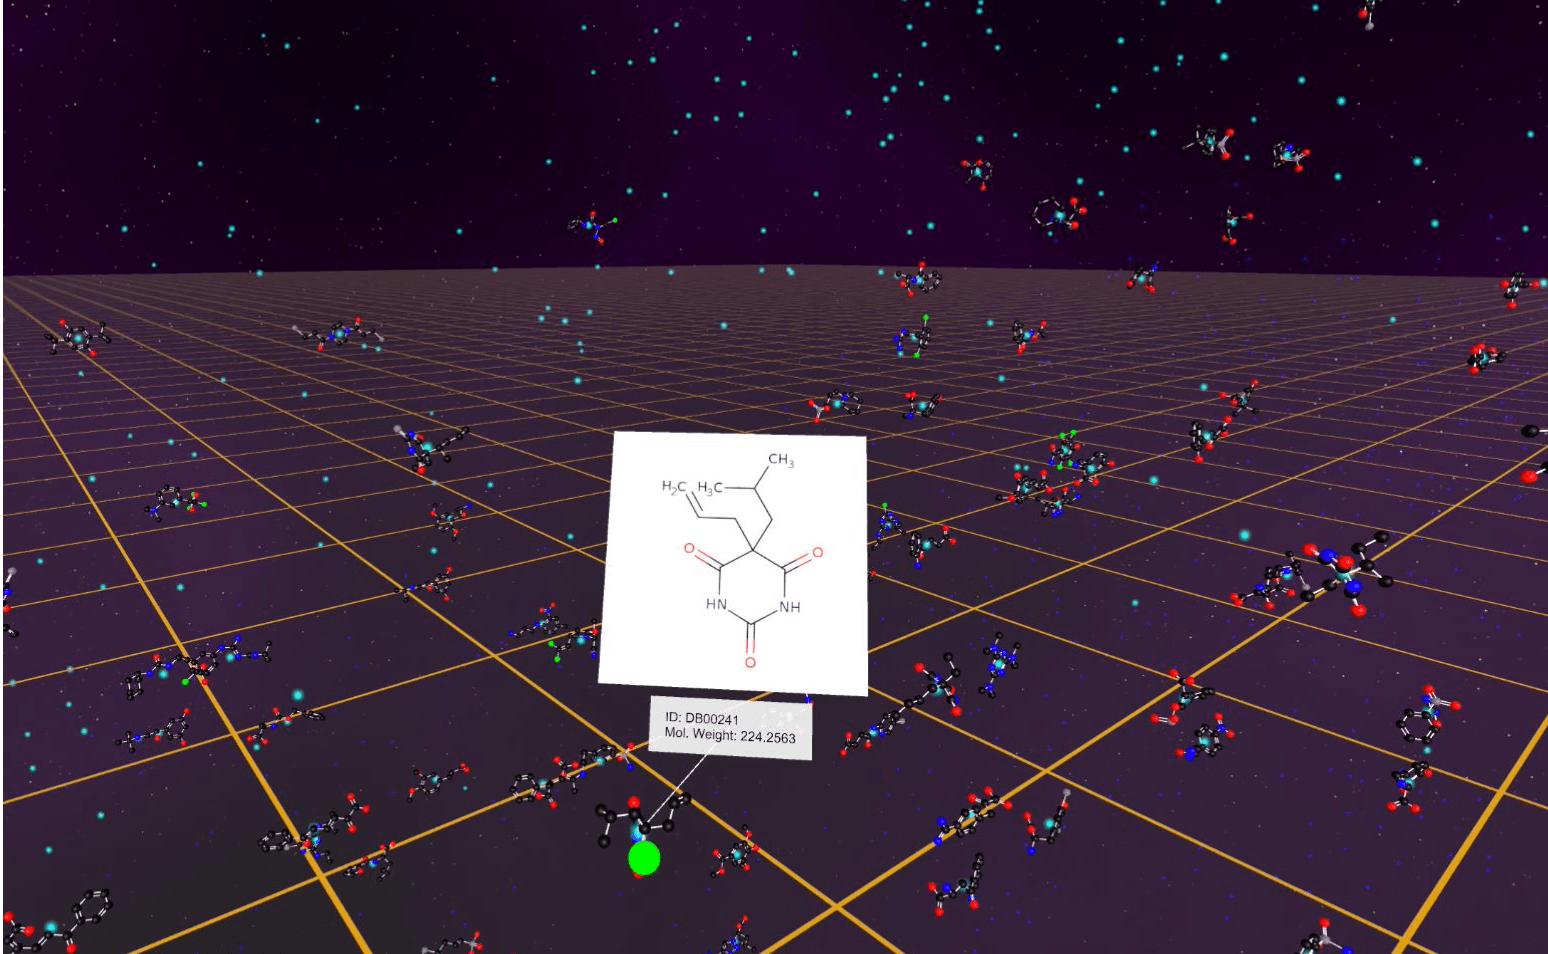
\includegraphics[width=\textwidth]{drugbank}
    \caption{Optimized virtual reality chemical space. Figure taken from \cite{drugbank}.}
    \label{fig:drugbank}
\end{figure}%

\section{BioVR}

\section{CellexaVR}

\section{BigTop}
